\begin{frame}{CDMX Covid-19 data}
    \begin{figure}[htb]
        \centering
        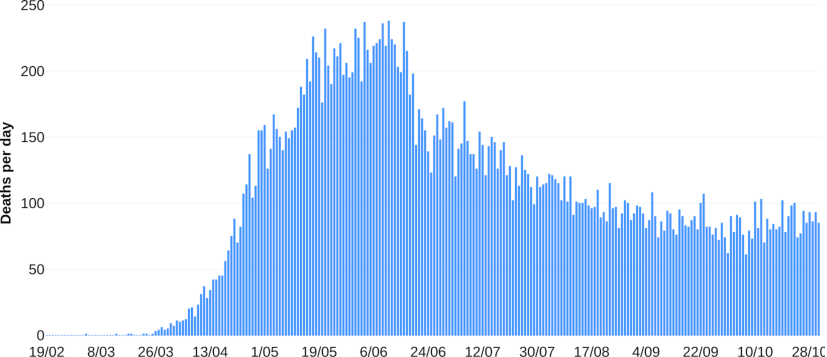
\includegraphics[width=0.8\textwidth, keepaspectratio]{%
            sto_mle_covid19/Figures/CDMX_dta.png%
        }
        \caption{%
            CDMX data
        }
        \label{fig:data_CDMX_fitting}
    \end{figure}
\end{frame}


\begin{frame}{An application to the estimation of parameters}
    \begin{Huge}
        \begin{description}
            \item[Example:]
                Estimation of the infection rates
                $\beta_s$, $\beta_a$, and ratio of asymptomatic cases $p$.
            \item[Argument:]
                Noise could improve the
                uncertainty quantification.
        \end{description}
    \end{Huge}
    \footnote{
        Work in progress. 
        \\ Somited in IJCM.
        Fernado Baltazar (UNAM-CU) and Francisco Delgado
        (CONACYT-UNAM-OAXACA)}
\end{frame}
%------------------------------------------------------------
\begin{frame}{MCMC with a deterministic SEIRS structure}
    \begin{textblock*}{120mm}(0mm, 10mm)
        \only<1->{        
            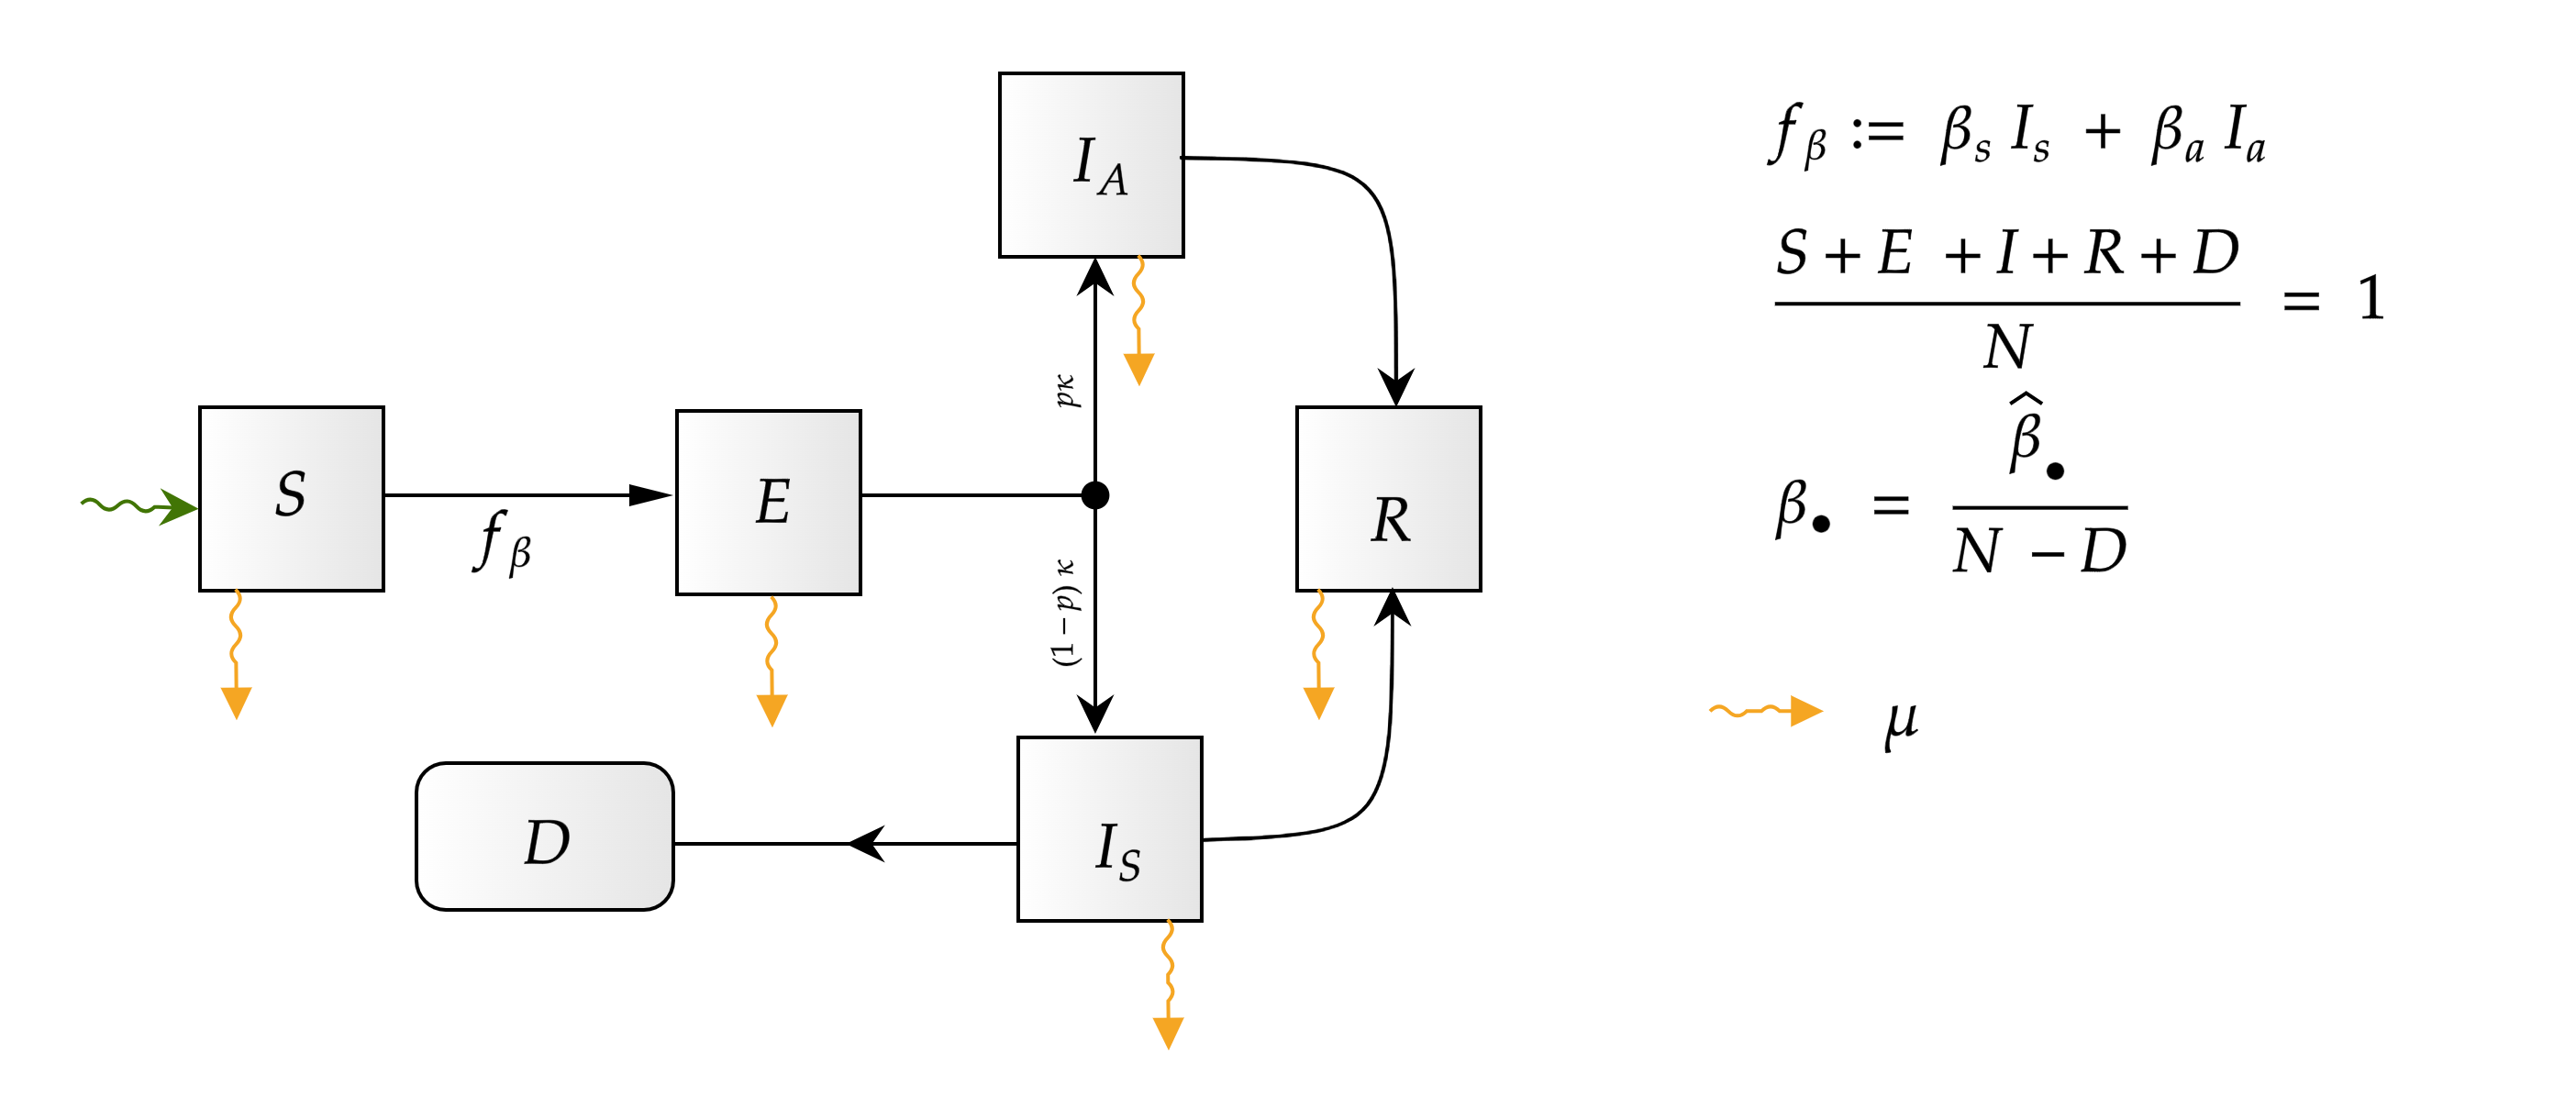
\includegraphics[width=\textwidth]{assets/stoSEIR_diagram.png} 
        }
    \end{textblock*}    
%    
%%    
    \begin{textblock*}{60mm}(0mm, 50mm)
	    \only<2->{
	        \begin{equation*}
	            \label{eqn:base_dynamics}
	            \begin{aligned}
	                S'  &=
	                    \mu +\gamma R
	                    - \left(\mu  + f_{\beta} \right)  S
	                \\
	                 E' & =  f_{\beta}S
	                     - (\kappa E + \mu E
	                     )
	                \\
	                {I_a}' &=
	                    p \kappa E
	                    - \big(\alpha_a + \mu \big)I_a
	                \\
	                 {I_s}' &=
	                    (1 - p) \kappa E
	                    - (\alpha_s +\mu)  I_s
	                \\
	                {R}' &=
	                    \alpha_a I_a + \alpha_s (1 - \theta)I_s -
	                    (\mu + \gamma) R
	                \\
	                D' &= \theta \alpha_s I_s.
	            \end{aligned}
	        \end{equation*}
	     }
    \end{textblock*}
%%    
    \begin{textblock*}{60mm}(65mm, 55mm)
	    \only<3>{
	        \begin{equation*}
	            \label{eqn:base_dynamics_counter}
	            \begin{aligned}
	                Y_t & \sim
	                    \mathrm{Poisson}(\lambda_t)
	                \\
	                    \lambda_t =& \int_0 ^ t (1-p) \kappa E
	                \\
	                    p & \sim
	                    \mathrm{Uniform}(0.3, 08)
	                \\
	                    \kappa & \sim
	                    \mathrm{Gamma}(10, 50)
	                \\
	                    \beta_a, \beta_s & \sim\mathcal{N}(0.5,0.1)    
	            \end{aligned}
	        \end{equation*}
	    }
    \end{textblock*}
\end{frame}
%%%%%%%%%%%%%%%%%%%%%%%%%%%%%%%%%%%%%%%%%%%%%%%%%%%%%%%%%%%%%%%%%%%%%%%%%%%%%%%%
\begin{frame}{Overfiting example}
    \begin{figure}[htb]
        \centering
        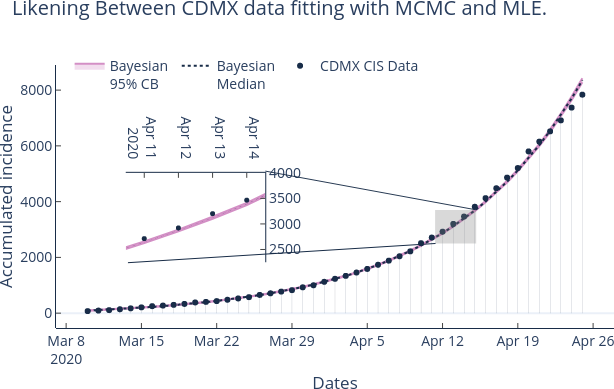
\includegraphics[width=0.8\textwidth, keepaspectratio]{%
            sto_mle_covid19/Figures/MCMC_CDMXDataFitting.png%
        }
        \caption{%
            MCMC Fit of diary new cases of Mexico city
            during exponential growth. See
            \url{https://plotly.com/~sauld/53/} for an electronic
            version.
        }
        \label{fig:data_CDMX_fitting}
    \end{figure}
\end{frame}